\documentclass[11pt]{article}
\usepackage[margin=1in]{geometry}
\usepackage{amsmath,amssymb}
\usepackage{booktabs}
\usepackage{array}
\usepackage{xcolor}
\usepackage[most]{tcolorbox}
\usepackage{enumitem}
\usepackage{tikz}
\usepackage{pifont}
\usetikzlibrary{arrows.meta,positioning,decorations.pathreplacing}
\usepackage[colorlinks=true,linkcolor=blue!50!black,urlcolor=blue!50!black,citecolor=blue!50!black]{hyperref}

\definecolor{accent}{RGB}{122,45,45}   % red  = learned morphing / family 2
\definecolor{famone}{RGB}{35,78,112}   % blue = family-1 nominal ratios / ridge
\definecolor{known}{RGB}{31,107,59}    % green = known a-priori rates
\definecolor{mut}{RGB}{107,107,107}

\newtcolorbox{takeaway}[1][]{colback=yellow!12,colframe=orange!70!black,
  title={#1},fonttitle=\bfseries,boxrule=0.6pt,arc=2pt,left=4pt,right=4pt,top=3pt,bottom=3pt}
\newtcolorbox{keybox}[1][]{colback=blue!4,colframe=blue!40!black,
  title={#1},fonttitle=\bfseries,boxrule=0.6pt,arc=2pt,left=4pt,right=4pt,top=3pt,bottom=3pt}
\newtcolorbox{qbox}[1][]{colback=black!3,colframe=black!35,
  title={#1},fonttitle=\bfseries\itshape,boxrule=0.5pt,arc=2pt,left=4pt,right=4pt,top=3pt,bottom=3pt}

\newcommand{\kl}{\ensuremath{\kappa_\lambda}}
\newcommand{\mhh}{\ensuremath{m_{HH}}}
\newcommand{\bbtt}{\ensuremath{b\bar b\tau\tau}}
\newcommand{\bbgg}{\ensuremath{b\bar b\gamma\gamma}}
\newcommand{\fourb}{\ensuremath{b\bar bb\bar b}}
\newcommand{\ahh}{\ensuremath{\hat{\hat\alpha}}}
\setlist{itemsep=2pt,topsep=3pt}

\title{\vspace{-2.5em}Lesson-1 Q\&A --- rates vs.\ morphing, profiling,\\
and the anatomy of learned ratios}
\author{\normalsize\itshape teaching companion note --- Q\&A of 11 July 2026, organized}
\date{11 July 2026}

\begin{document}
\maketitle
\vspace{-1.6em}

\begin{takeaway}[What this note is]
A cleaned-up, \emph{complete} record of the Q\&A session revisiting
\href{../lessons/0001-nsbi-systematics-field-map.html}{Lesson 1} (the NSBI-systematics field map), grouped
logically rather than chronologically. Part~\ref{sec:anatomy}: what in the likelihood is \emph{known a priori}
vs.\ \emph{learned}, and what the learned objects actually are (the green rate factor; weights vs.\ density
ratios; \kl-independence; the per-event anchor construction). Part~\ref{sec:profiling}: what profiling is and
exactly how a tilted \kl--$\alpha$ likelihood widens the confidence interval, plus the meaning of the profile
likelihood ratio $\lambda(\kl)$. Part~\ref{sec:assumptions}: the four off-shell (R2) modeling assumptions
unpacked, and how each breaks in \bbtt, \bbgg, and \fourb. Part~\ref{sec:upgrades}: how R3 (Gaussian-Process
morphing) and R4 (the ``refinable'' surrogate) relax those assumptions --- including the verified correction that
R4 is \emph{not} a generative/normalizing-flow method. Companion to the \kl-challenges note
(\texttt{2026-06-20-klambda-nsbi-vs-offshell-challenges}); challenge labels C1--C6 refer to its Sec.~5.
\end{takeaway}

\tableofcontents

%=====================================================================
\section{The model's anatomy: what is known, what is learned}\label{sec:anatomy}

\subsection{``The green factor $\kappa$ (rates) has a \emph{known a-priori} dependence''}\label{sec:green}

\begin{qbox}[Question]
Can you elaborate ``The green factor $\kappa$ (rates: lumi, cross-section, POIs) has a known a-priori
dependence''?
\end{qbox}

In the Lesson-1 master equation, each sample $s$ contributes a product of four factors, and the color-coding
splits them by \emph{where the parameter-dependence comes from}:
\begin{equation}
P(x\,|\,\eta,\chi)\;\propto\;\prod_{\text{events }e}\Big[\sum_{\text{samples }s}
\nu_s(\eta,\xi)\cdot{\color{known}\kappa_s(\eta,\xi)}\cdot
{\color{accent}\boldsymbol{\Delta_s(x_e\,|\,\alpha)}}\cdot P_s(x_e)\Big]\cdot\prod_p f(a_p|\chi_p),
\end{equation}
with $\eta$ the POIs, $\xi$ unconstrained normalization parameters, $\alpha$ the constrained nuisance
parameters, and the last factor the Gaussian constraint terms.
\begin{itemize}
\item $P_s(x)$ --- the \emph{nominal} per-event shape of sample $s$. Fixed; learned once (the ratio network at
  $\alpha=0$).
\item $\nu_s\cdot{\color{known}\kappa_s}$ (\textcolor{known}{\textbf{green}}) --- the \emph{expected event
  count} of sample $s$ and its multiplicative rate modifiers: yield $=$ luminosity $\times$ cross-section
  $\times$ efficiency, scaled by the POI and by normalization nuisances.
\item ${\color{accent}\Delta_s(x|\alpha)}$ (\textcolor{accent}{\textbf{red}}) --- how the \emph{shape} deforms
  when a systematic is dialed.
\end{itemize}

\noindent``Known a-priori'' means: for every parameter entering the green factor, the functional form is
something you can \textbf{write down in closed form before touching any simulation}, with exact derivatives ---
there is nothing to learn:
\begin{itemize}
\item \textbf{Luminosity.} The yield scales \emph{linearly} in $L$ ($\nu\propto L$); a $\pm1.6\%$ lumi NP
  multiplies every MC sample's rate by the log-normal $e^{\alpha\sigma_{\ln}}$. Pure bookkeeping.
\item \textbf{Cross-section / normalization NPs.} The same closed log-normal form, per process.
\item \textbf{POIs.} For the off-shell measurement, the mixture coefficients
  $(\mu-\sqrt\mu,\ \sqrt\mu,\ 1-\sqrt\mu)$ are exact functions of $\mu$ from the amplitude structure. For \kl:
\begin{equation}
\sigma(\kl)\;=\;\kl^2\,A\;+\;\kl\,B\;+\;C,
\end{equation}
  an \emph{exact parabola} from $|\kl\cdot\text{triangle}+\text{box}|^2$; simulation only supplies the three
  constants $A,B,C$.
\end{itemize}

The deeper point for \kl: \textbf{even the POI's \emph{shape} dependence is handled a-priori} via the mixture
trick. One never learns ``how the shape morphs with \kl'' --- the signal is split into three fixed-shape
components ($|\text{triangle}|^2$, interference, $|\text{box}|^2$) with fixed $P_s(x)$, and \emph{all}
\kl-dependence lives in the known green coefficients $(\kl^2,\ \kl,\ 1)$. The learning budget is reserved for
the red factor --- the systematics --- where no amplitude-level decomposition exists: the $\alpha$-dependence of
the shape emerges from the shower$\to$detector$\to$reconstruction chain, has no closed form, and is intractable.
That asymmetry --- \textbf{POI dependence by construction, nuisance dependence by learning} --- is the core
architecture of the whole method.

\begin{keybox}[Caveat: the green/red boundary is where C4 lives]
The green/red split is a \emph{modeling choice}, and it can be wrong. \texttt{THU\_HH} is naively filed under
green (a $\pm$lnN rate modifier), but faithfully it is \kl-dependent \emph{and} shape-bearing (the three signal
components carry different theory bands) --- so it leaks across the boundary into red and, worse, couples
POI$\times$nuisance. ``Which factor does this NP really belong in?'' is a useful discipline for every
systematic in the table.
\end{keybox}

%---------------------------------------------------------------------
\subsection{Weights \emph{are} density ratios: the two learned families}\label{sec:families}

\begin{qbox}[Question]
We've been talking about learning density ratios --- what do you mean by learning a \emph{weight per
component}?
\end{qbox}

The two phrases sound like different machinery, and they are not. \textbf{A ``weight'' \emph{is} a learned
density ratio.} The only thing that changes is \emph{which two densities} sit in the ratio. The full NSBI model
contains \textbf{two families of learned ratios}, distinguished purely by their numerator/denominator
(Fig.~\ref{fig:families}):

\begin{figure}[htbp]\centering
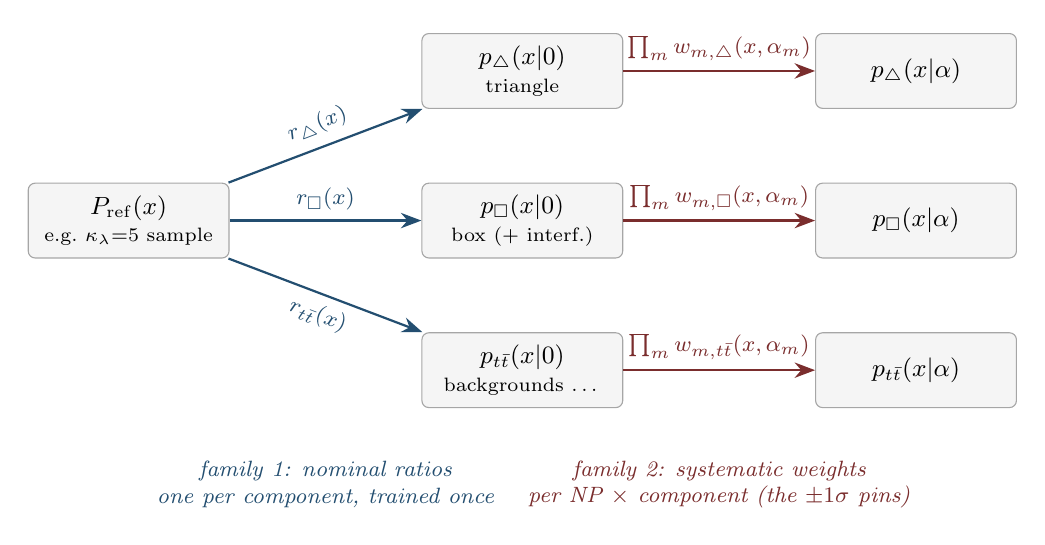
\begin{tikzpicture}[
  box/.style={draw=black!35, fill=black!4, rounded corners=2.5pt, minimum width=2.55cm, minimum height=0.95cm,
              align=center, font=\small},
  lab/.style={font=\footnotesize\itshape},
  arr1/.style={-{Stealth[length=2.6mm]}, famone, thick},
  arr2/.style={-{Stealth[length=2.6mm]}, accent, thick}]
  % reference
  \node[box] (ref) at (0,0) {$P_{\rm ref}(x)$\\[-1pt]{\scriptsize e.g.\ $\kl{=}5$ sample}};
  % component nominals
  \node[box] (tri) at (5.0, 1.9) {$p_\triangle(x|0)$\\[-1pt]{\scriptsize triangle}};
  \node[box] (bx)  at (5.0, 0.0) {$p_\square(x|0)$\\[-1pt]{\scriptsize box ($+$ interf.)}};
  \node[box] (tt)  at (5.0,-1.9) {$p_{t\bar t}(x|0)$\\[-1pt]{\scriptsize backgrounds \dots}};
  % varied
  \node[box] (triV) at (10.0, 1.9) {$p_\triangle(x|\alpha)$};
  \node[box] (bxV)  at (10.0, 0.0) {$p_\square(x|\alpha)$};
  \node[box] (ttV)  at (10.0,-1.9) {$p_{t\bar t}(x|\alpha)$};
  % family 1 arrows
  \draw[arr1] (ref) -- (tri) node[midway, above, sloped, lab, famone]{$r_\triangle(x)$};
  \draw[arr1] (ref) -- (bx)  node[midway, above, lab, famone]{$r_\square(x)$};
  \draw[arr1] (ref) -- (tt)  node[midway, below, sloped, lab, famone]{$r_{t\bar t}(x)$};
  % family 2 arrows
  \draw[arr2] (tri) -- (triV) node[midway, above, lab, accent]{$\prod_m w_{m,\triangle}(x,\alpha_m)$};
  \draw[arr2] (bx)  -- (bxV)  node[midway, above, lab, accent]{$\prod_m w_{m,\square}(x,\alpha_m)$};
  \draw[arr2] (tt)  -- (ttV)  node[midway, above, lab, accent]{$\prod_m w_{m,t\bar t}(x,\alpha_m)$};
  % family labels
  \node[lab, famone, align=center] at (2.5,-3.35) {family 1: nominal ratios\\ one per component, trained once};
  \node[lab, accent, align=center] at (7.5,-3.35) {family 2: systematic weights\\ per NP $\times$ component (the $\pm1\sigma$ pins)};
\end{tikzpicture}
\caption{The two families of learned density ratios. Every arrow is the \emph{same kind of object} --- a density
ratio learned by a classifier --- differing only in which two samples it compares. The mixture then combines
components with the \textcolor{known}{known} coefficients:
$\nu(x;\kl,\alpha)=\sum_s {\color{known}c_s(\kl)}\,\nu_s\,{\color{famone}r_s(x)}
\,{\color{accent}\prod_m w_{m,s}(x,\alpha_m)}\,P_{\rm ref}(x)$, with $c_s=(\kl^2,\kl,1,\dots)$.}
\label{fig:families}
\end{figure}

\begin{table}[htbp]\centering\small
\begin{tabular}{@{}p{0.185\textwidth}p{0.36\textwidth}p{0.37\textwidth}@{}}
\toprule
 & \textbf{Family 1: nominal ratio $r_s(x)$} & \textbf{Family 2: systematic weight $w_{m,s}(x,\alpha_m)$}\\
\midrule
the ratio & $p_s(x|\alpha{=}0)\;/\;P_{\rm ref}(x)$ & $p_s(x|\alpha_m{=}{\pm}1)\;/\;p_s(x|\alpha{=}0)$\\
compares & \emph{different components}, both nominal & \emph{the same component}, varied vs nominal\\
trained by & classifier: component-$s$ sample \textbf{vs reference} $\to s/(1{-}s)$ & classifier: $\pm1\sigma$-varied
  sample of $s$ \textbf{vs nominal} of $s$ $\to s/(1{-}s)$\\
carries & the physics separation (\kl\ info via the mixture) & the systematic deformation (the $\alpha$-dependence)\\
how many & one per component ($\sim$5--7) & $2\times N_{\rm NP}\times N_{\rm comp}$ ($\sim$thousands) --- this is C2\\
typical size & can be large/structured (different processes) & $\approx1$ everywhere (varied $\approx$ nominal):
  small multiplicative corrections\\
\bottomrule
\end{tabular}
\caption{Same trick, different sample pairs.}
\label{tab:families}
\end{table}

``Learning a weight per component'' therefore means: for one NP, say JES, one trains a separate Family-2 ratio
for each middle-column box of Fig.~\ref{fig:families} --- one classifier for (JES$+1\sigma$ triangle vs.\
nominal triangle), another for the box component, another for $t\bar t$, and so on. Each is a density ratio in
exactly the sense used throughout. The pins of Sec.~\ref{sec:pins} are the \emph{values of one Family-2 ratio at
$\alpha=\pm1$} for one event.

\paragraph{Why it is called a ``weight'' rather than a ``ratio''.} Because of how it is \emph{used}:
multiplying the nominal density by it \emph{is} per-event reweighting --- event $e$, carrying weight
$w(x_e,\alpha)$, emulates the varied sample without regenerating it (the CARL/DCTR reweighting sense of
Lesson~7). Mathematically a ratio; operationally a weight. The chain composes by multiplication:
\begin{equation}
p_s(x|\alpha)\;=\;{\color{accent}w_s(x,\alpha)}\cdot p_s(x|0)
\;=\;{\color{accent}w_s(x,\alpha)}\cdot{\color{famone}r_s(x)}\cdot P_{\rm ref}(x)
\end{equation}
--- two hops: reference $\to$ component nominal (blue, Family 1), then nominal $\to$ varied (red, Family 2).

\paragraph{Why factor into two hops instead of learning $p_s(x|\alpha)/P_{\rm ref}$ directly as one
$\alpha$-parameterized ratio?} Three practical reasons:
\begin{enumerate}
\item \textbf{Statistics where the danger is.} \emph{(Wording sharpened after a learner catch --- record 0011:
  ``easy/hard'' here means ratio-\emph{estimation} difficulty, which runs \emph{opposite} to classification
  difficulty.)} For \emph{classification}, separation is fuel: different distributions $=$ easy (high AUC),
  similar $=$ hard (AUC $\approx0.5$, weak gradients). But the fit consumes the \emph{value} of $r=s/(1-s)$,
  not the ranking --- and for the value, the difficulty inverts. The \textbf{Family-1} ratio is hard in the
  \emph{dangerous} sense: the target spans orders of magnitude and is unbounded where the reference support
  thins; the sigmoid saturates exactly where the value matters; calibration errors multiply the entire density.
  It therefore gets the ample nominal MC ($\approx$500--750k events per \kl\ point) and is trained \emph{once}.
  The \textbf{Family-2} ratios are \emph{feasible-by-construction}: the target is a bounded, perturbative
  correction around $w\equiv1$, and the failure mode is graceful --- an under-trained net collapses toward
  $w=1$, a few-percent absolute error that \emph{understates a systematic} rather than corrupting the density.
  That boundedness is what makes them learnable at all from the smaller $\pm1\sigma$ samples.
  \emph{Caveat --- the C6 burden:} on those small samples the training \emph{noise} on the few-percent deviation
  can rival the deviation itself, and a net can latch onto the sample's own fluctuations; this is a real
  hardness, but of the \emph{variance} kind --- quantifiable and insurable (ensembles, C2ST checks, the wifi
  band) --- not an intractability. Asking a small sample to support a Family-1-style unbounded ratio directly
  (the one-hop alternative) would be \emph{both} problems at once, with the catastrophic failure mode.
\item \textbf{Modularity.} Adding, dropping, or retraining an NP never touches the nominal ratios or any other
  NP's weights.
\item \textbf{It is the factorization ansatz made flesh} --- one Family-2 curve per NP, multiplied --- with all
  the costs discussed in Sec.~\ref{sec:assumptions}.
\end{enumerate}

\paragraph{Anchor in the project's own code.} The preliminary analysis (\texttt{DiHiggs\_Lambda\_NSBI}) has
built \textbf{only Family 1} --- the ensembles of per-basis-sample and per-background ratios against the
$\kl{=}5$ reference. It has zero Family-2 objects, which is precisely the operational meaning of ``no
systematic NPs in the fit yet.'' The systematics program (C1/C2/C5/C6) is, concretely, the project of standing
up the red-arrow family --- thousands of near-unity ratios --- and controlling their interpolation, cross-terms,
and MC-statistical noise.

%---------------------------------------------------------------------
\subsection{Are the weights \kl-independent? (yes --- with one sharpening)}\label{sec:lambdaindep}

\begin{qbox}[Question]
Most systematics weights are $\lambda$-independent (except the theory systematics), right?
\end{qbox}

Yes --- and by \emph{design}, not by accident. In the factorized scheme every systematic weight takes only
$(x,\alpha_m)$ as arguments; \kl\ never appears inside any of them. The \kl-dependence of the \emph{total}
prediction lives entirely upstairs, in the known mixture coefficients:
\begin{equation}
\nu(x;\kl,\alpha)\;=\;\sum_{\text{components }s}{\color{known}c_s(\kl)}\cdot\nu_s\cdot
\big[\text{nominal ratio}_s(x)\big]\cdot{\color{accent}\prod_m w_{m,s}(x,\alpha_m)},\qquad
c_s=(\kl^2,\ \kl,\ 1).
\end{equation}

For \textbf{experimental} NPs this \kl-independence is \emph{physically correct} --- the detector does not know
the coupling; a $+1\sigma$ JES miscalibration does the same thing to a given event whatever \kl\ is. But note
the load-bearing subtlety: \textbf{this only holds because the weights are learned per component.} JES deforms
the triangle, box, and interference densities \emph{differently} (they have different \mhh\ spectra), so each
component carries its own $w$. The net JES effect on the \emph{summed} signal then automatically inherits the
right \kl-dependence through the mixture. If one instead trained a single JES weight on a fixed-\kl\ total
mixture (say the SM one), it would be silently wrong at $\kl=5$ --- a hidden $\lambda$-dependence smuggled in by
implementation. That is why ATLAS trains $2\times N_{\rm NP}\times$\emph{process} (signal components counted
separately), and why the preliminary setup trains ratios per basis sample.

The \textbf{theory} NP is the one place where this clean structure genuinely fails \emph{as prescribed} ---
because the uncertainty is only \emph{given} at the total-signal level ($+4/{-}18\%$ \emph{at the SM point}),
with a \kl-dependent size and composition. Faithfulness then forces either the per-component decomposition
(which restores $\alpha$-only weights but needs the unpublished component-differential bands) or an explicitly
\kl-dependent weight $w_\theta(x;\kl,\alpha_\theta)$ --- that is exactly challenge C4.

%---------------------------------------------------------------------
\subsection{``Pinned by two numbers, threaded through a fixed smooth family''}\label{sec:pins}

\begin{qbox}[Question]
What do you mean by ``The entire $\alpha$-dependence of each event's weight is then pinned by just those two
numbers, threaded through a fixed smooth family''?
\end{qbox}

This sentence is about a \textbf{single event's weight as a function of $\alpha$} --- nothing to do with \kl.
Fix one NP (say $\tau$ES), one component $s$, one event $x_e$ (Fig.~\ref{fig:pins}):
\begin{enumerate}
\item \textbf{What is actually trained:} two classifiers --- ($+1\sigma$ sample vs nominal) and ($-1\sigma$
  sample vs nominal). Via $s/(1{-}s)$ they yield two per-event numbers:
\begin{equation}
w_+(x_e)=\frac{p(x_e|\alpha{=}{+}1)}{p(x_e|\alpha{=}0)},\qquad
w_-(x_e)=\frac{p(x_e|\alpha{=}{-}1)}{p(x_e|\alpha{=}0)}.
\end{equation}
For the drawn event: $w_+=1.20$, $w_-=0.85$ --- ``a $+1\sigma$ $\tau$ES makes events \emph{like this one} 20\%
more likely.''
\item \textbf{What the fit needs:} $w(x_e,\alpha)$ at \emph{every} $\alpha$, because the minimizer explores
  $\alpha$ continuously ($0.37$, $-1.6$, \dots) while profiling.
\item \textbf{The bridge:} through the three known points $(-1,\,w_-)$, $(0,\,1)$, $(+1,\,w_+)$, draw a curve
  from a \textbf{fixed, pre-chosen family} --- the HistFactory ``poly-exp'': exponential in the tails
  ($w_+^{\,\alpha}$ for $\alpha>1$, so $\alpha{=}{+}2\Rightarrow1.20^2=1.44$; $w_-^{\,|\alpha|}$ for
  $\alpha<-1$), and for $|\alpha|<1$ a 6th-order polynomial whose coefficients are \emph{fully determined} by
  smoothly matching the tails (value, first and second derivative) at $\pm1$. \textbf{Zero free parameters
  remain.} At $\alpha=0.5$ the curve gives $\approx w_+^{0.5}\approx1.10$ for well-behaved anchors (the interior
  polynomial hugs the exponential).
\end{enumerate}
That is the sentence: once $w_+(x_e)$ and $w_-(x_e)$ are known, the \emph{entire function of $\alpha$} for this
event is decided --- the event's kinematics enter only through where the two pins sit; the \emph{shape of the
path between and beyond the pins} is universal, identical for every event, every NP, every analysis.

\begin{figure}[htbp]\centering
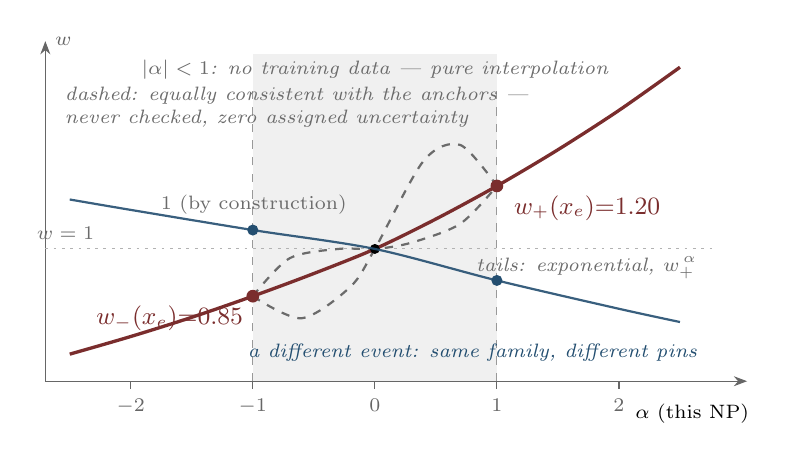
\begin{tikzpicture}[x=1.55cm, y=4.0cm]
  % interior band
  \fill[black!6] (-1,-0.42) rectangle (1,0.62);
  \node[font=\scriptsize\itshape, text=mut] at (0,0.57) {$|\alpha|<1$: no training data --- pure interpolation};
  % axes
  \draw[-{Stealth}, black!60] (-2.7,-0.42) -- (3.05,-0.42);
  \node[below, font=\scriptsize] at (2.6,-0.46) {$\alpha$ (this NP)};
  \draw[-{Stealth}, black!60] (-2.7,-0.42) -- (-2.7,0.66) node[right, font=\scriptsize]{$w$};
  \foreach \a in {-2,-1,0,1,2}{\draw[black!60] (\a,-0.42) -- (\a,-0.445) node[below, font=\scriptsize]{$\a$};}
  \draw[black!30, dash pattern=on 1pt off 2pt] (-2.7,0) -- (2.8,0) node[pos=0.03, above, font=\scriptsize, text=mut]{$w=1$};
  % anchor verticals
  \draw[black!40, dashed] (-1,-0.42) -- (-1,0.52);
  \draw[black!40, dashed] (1,-0.42) -- (1,0.52);
  % alternatives (interior only), through (-1,-.15),(0,0),(1,.20)
  \draw[mut, dashed, thick] plot[smooth] coordinates {(-1,-0.15) (-0.6,-0.22) (-0.2,-0.12) (0,0) (0.4,0.28) (0.7,0.33) (1,0.20)};
  \draw[mut, dashed, thick] plot[smooth] coordinates {(-1,-0.15) (-0.7,-0.03) (-0.3,0.00) (0,0) (0.3,0.02) (0.7,0.08) (1,0.20)};
  \node[font=\scriptsize\itshape, text=mut, align=left, anchor=west] at (-2.62,0.45)
    {dashed: equally consistent with the anchors ---\\ never checked, zero assigned uncertainty};
  % main curve: w-=0.85, w+=1.20 => plot (alpha, w-1)
  \draw[accent, very thick] plot[smooth] coordinates
    {(-2.5,-0.334) (-2,-0.278) (-1.5,-0.217) (-1,-0.15) (-0.5,-0.078) (0,0) (0.5,0.095) (1,0.20) (1.5,0.315) (2,0.44) (2.5,0.577)};
  \fill[accent] (-1,-0.15) circle (2.3pt) node[below left, font=\small\itshape, text=accent]{$w_-(x_e){=}0.85$};
  \fill[black]  (0,0)      circle (1.8pt);
  \node[anchor=east, font=\scriptsize, text=mut] at (-0.15,0.14) {$1$ (by construction)};
  \fill[accent] (1,0.20)   circle (2.3pt);
  \node[anchor=west, font=\small\itshape, text=accent] at (1.06,0.13) {$w_+(x_e){=}1.20$};
  \node[font=\scriptsize\itshape, text=mut, anchor=east] at (2.72,-0.06) {tails: exponential, $w_+^{\,\alpha}$};
  % second event: w-=1.06, w+=0.90
  \draw[famone, thick, opacity=0.9] plot[smooth] coordinates
    {(-2.5,0.157) (-2,0.124) (-1,0.06) (0,0) (1,-0.10) (2,-0.19) (2.5,-0.232)};
  \fill[famone] (-1,0.06) circle (2pt);
  \fill[famone] (1,-0.10) circle (2pt);
  \node[font=\scriptsize\itshape, text=famone, anchor=east] at (2.72,-0.33) {a different event: same family, different pins};
\end{tikzpicture}
\caption{One event, one NP: two learned numbers $\Rightarrow$ the entire $\alpha$-curve. The $x$-dependence
lives only in where the pins sit; the path between and beyond them is a universal, pre-chosen family. The
dashed curves pass through the \emph{same} three points --- the training is equally happy with them --- yet they
would give different weights at $\alpha=0.5$, different profiled likelihoods, and different \kl\ intervals.}
\label{fig:pins}
\end{figure}

\noindent The dashed alternatives are the point of the whole critique: the method does not just pick one curve,
it picks one \textbf{and assigns zero uncertainty to the choice}. The R2 critique items of
Sec.~\ref{sec:assumptions} now become concrete:
\begin{itemize}
\item \textbf{``Fixed order in $\alpha$''} $=$ this family. It is smooth and monotone between the anchors by
  construction --- if the true per-event response is non-monotone (the dashed dipping curve; think of an event
  near a selection or SVfit threshold that migrates in and then out), the family \emph{cannot represent it}, at
  any anchor values.
\item \textbf{``Ignores kinematics for $|\alpha|<1$''} $=$ the shaded band. No simulation ever constrains the
  interior path. Sharper: if a sample were \emph{generated} at $\alpha=0.5$, this construction has \textbf{no
  slot to use it} --- the family is already fully pinned by $\pm1$. (R4's joint parametric fit would simply add
  it to the loss; R3's GP would take it as another anchor \emph{and} shrink its uncertainty band there.)
\item \textbf{Per-NP independence} of these curves (one such plot per NP, multiplied together) is the
  factorization assumption; each pin-pair being trained in isolation is the ``no joint likelihood ratios''
  point, with its C6 noise.
\end{itemize}
Connecting back to Sec.~\ref{sec:lambdaindep}: \kl\ appears nowhere in Fig.~\ref{fig:pins} --- that is the
$\lambda$-independence made visible. The figure is drawn \emph{per component}; the fit holds $\sim$dozens of
such pin-pairs per event (one per NP $\times$ component), multiplies them, and mixes components with the known
\kl\ coefficients. C4 is precisely the statement that for \texttt{THU\_HH} no single such $\lambda$-blind curve
can be faithful --- the \emph{pins themselves} would have to move as \kl\ changes, unless the theory band is
first decomposed per component.

%=====================================================================
\section{Profiling and the confidence interval}\label{sec:profiling}

\subsection{What ``profiling'' means}\label{sec:profdef}

\begin{qbox}[Question]
Can you remind me what exactly `profiling' means?
\end{qbox}

The full likelihood, with POI \kl\ and nuisances $\alpha$ (extended form, Gaussian constraints):
\begin{equation}
L(\kl,\alpha)\;=\;e^{-\nu_{\rm tot}(\kl,\alpha)}\prod_{e}\nu(x_e;\kl,\alpha)\;\times\;
\prod_m \mathcal N\!\big(a_m\,\big|\,\alpha_m,\,1\big).
\end{equation}
\textbf{Profiling} $=$ re-fit the nuisances at each fixed \kl:
\begin{equation}
\ahh(\kl)\;=\;\arg\max_\alpha\;L(\kl,\alpha)
\qquad\text{(``double-hat'': the systematics' \emph{best attempt to explain the data} given that \kl).}
\end{equation}
The \textbf{profile likelihood ratio} and test statistic:
\begin{equation}
\lambda(\kl)\;=\;\frac{L\big(\kl,\ \ahh(\kl)\big)}{L\big(\hat\kl,\ \hat\alpha\big)},\qquad
t(\kl)\;=\;-2\ln\lambda(\kl),
\end{equation}
with the denominator the global best fit (single hats). Confidence intervals:
$\mathrm{CI}_{68}=\{\kl: t\le1\}$, $\mathrm{CI}_{95}=\{\kl: t\le3.84\}$ (Wilks: $t\sim\chi^2_1$).

\medskip
The intuition in one paragraph: \textbf{profiling is a structured ``devil's advocate.''} For every candidate
\kl\ one asks: \emph{if this were the true coupling, how well could the systematics conspire to explain my data
anyway?} --- and one lets them try (that is the re-fit, $\ahh(\kl)$). A systematic costs sensitivity
\textbf{exactly to the extent it can mimic the POI} --- the tilt of the likelihood contours in the
$(\kl,\alpha)$ plane, which is the same $\rho(\kl,\alpha)$ as in the degeneracy toy. No tilt $\to$ profiling
changes nothing; strong tilt (JES/$\tau$ES on \mhh) $\to$ the parabola flattens and the CI widens. The width
quoted is the \emph{honest} one: it already includes every way the nuisances could have fooled you, weighted by
their constraints.

%---------------------------------------------------------------------
\subsection{Reading the widening off the picture: slice vs.\ shadow}\label{sec:slice}

\begin{qbox}[Question]
How to read off how the widening happens through profiling in the tilted case?
\end{qbox}

The key reframe: \textbf{the ellipse is a single fixed object} (the $t{=}1$ contour of the full 2-D
likelihood). ``Frozen'' and ``profiled'' are two different ways of extracting a 1-D interval from it
(Fig.~\ref{fig:slice}):
\begin{itemize}
\item \textbf{Frozen $\alpha$} $=$ the \textbf{central horizontal slice}: walk left/right from the minimum
  along the line $\alpha=\hat\alpha$ and mark where you exit the contour.
\item \textbf{Profiled} $=$ the \textbf{shadow} (projection) of the whole ellipse onto the \kl\ axis: the
  extreme left/right points reached \emph{anywhere} on the contour.
\end{itemize}
A slice can never be longer than the shadow --- and they are equal exactly when the ellipse is axis-aligned.
\textbf{The tilt is the entire effect.}

\begin{figure}[htbp]\centering
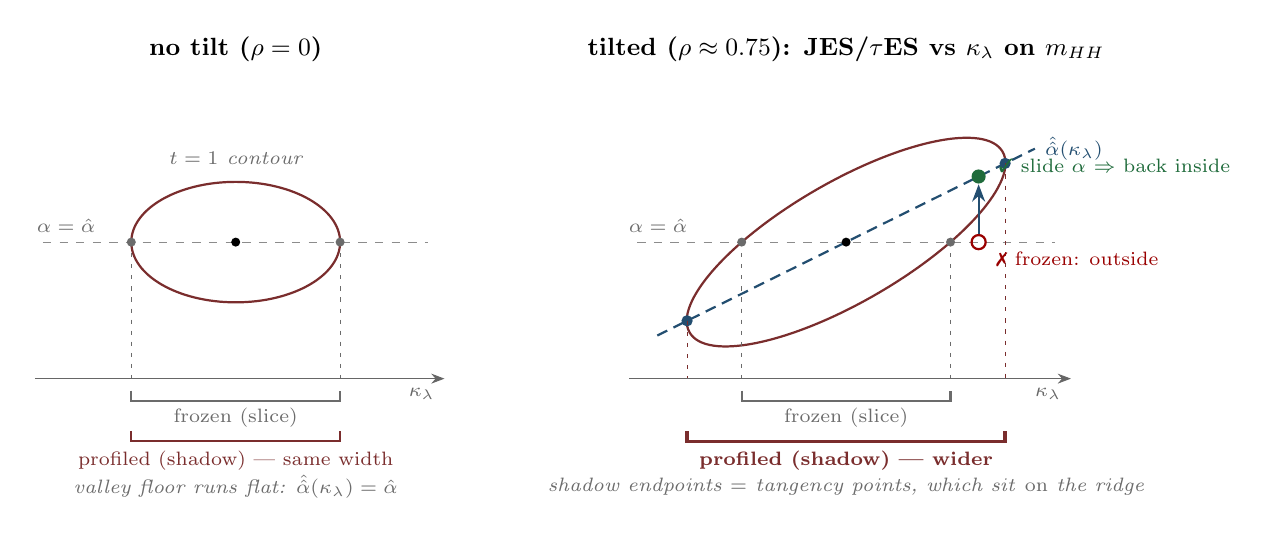
\begin{tikzpicture}[scale=1.02]
  %------------ panel A: no tilt ------------
  \begin{scope}[shift={(0,0)}]
    \node[font=\small\bfseries] at (0,2.4) {no tilt ($\rho=0$)};
    \draw[black!45, dash pattern=on 3pt off 3pt] (-2.4,0) -- (2.4,0) node[pos=0.06, above, font=\scriptsize, text=mut]{$\alpha=\hat\alpha$};
    \draw[accent, thick] (0,0) ellipse [x radius=1.30, y radius=0.75];
    \node[font=\scriptsize\itshape, text=mut] at (0,1.05) {$t=1$ contour};
    \fill (0,0) circle (1.6pt);
    \fill[mut] (-1.30,0) circle (1.6pt); \fill[mut] (1.30,0) circle (1.6pt);
    \draw[mut, dash pattern=on 1.5pt off 2.5pt] (-1.30,0) -- (-1.30,-1.7);
    \draw[mut, dash pattern=on 1.5pt off 2.5pt] (1.30,0) -- (1.30,-1.7);
    \draw[-{Stealth}, black!60] (-2.5,-1.7) -- (2.6,-1.7) node[below left, font=\scriptsize]{\kl};
    \draw[mut, thick] (-1.30,-1.85) -- ++(0,-0.13) -- ++(2.60,0) -- ++(0,0.13);
    \node[font=\scriptsize, text=mut] at (0,-2.18) {frozen (slice)};
    \draw[accent, thick] (-1.30,-2.35) -- ++(0,-0.13) -- ++(2.60,0) -- ++(0,0.13);
    \node[font=\scriptsize, text=accent] at (0,-2.72) {profiled (shadow) --- same width};
    \node[font=\scriptsize\itshape, text=mut] at (0,-3.05) {valley floor runs flat: $\ahh(\kl)=\hat\alpha$};
  \end{scope}
  %------------ panel B: tilted ------------
  \begin{scope}[shift={(7.6,0)}]
    \node[font=\small\bfseries] at (0,2.4) {tilted ($\rho\approx0.75$): JES/$\tau$ES vs \kl\ on \mhh};
    \draw[black!45, dash pattern=on 3pt off 3pt] (-2.6,0) -- (2.6,0) node[pos=0.05, above, font=\scriptsize, text=mut]{$\alpha=\hat\alpha$};
    % ridge: slope 0.495
    \draw[famone, thick, dash pattern=on 4pt off 2.5pt] (-2.35,-1.163) -- (2.35,1.163)
      node[right, font=\scriptsize\itshape, text=famone]{$\ahh(\kl)$};
    \draw[accent, thick, rotate=30] (0,0) ellipse [x radius=2.25, y radius=0.75];
    \fill (0,0) circle (1.6pt);
    % slice endpoints (half-length 1.30)
    \fill[mut] (-1.30,0) circle (1.6pt); \fill[mut] (1.30,0) circle (1.6pt);
    \draw[mut, dash pattern=on 1.5pt off 2.5pt] (-1.30,0) -- (-1.30,-1.7);
    \draw[mut, dash pattern=on 1.5pt off 2.5pt] (1.30,0) -- (1.30,-1.7);
    % tangency points (±1.98, ±0.98) on ridge
    \fill[famone] (1.98,0.98) circle (2pt); \fill[famone] (-1.98,-0.98) circle (2pt);
    \draw[accent, dash pattern=on 1.5pt off 2.5pt] (1.98,0.98) -- (1.98,-1.7);
    \draw[accent, dash pattern=on 1.5pt off 2.5pt] (-1.98,-0.98) -- (-1.98,-1.7);
    % test point A frozen (outside), B on ridge (inside)
    \draw[red!60!black, thick] (1.65,0) circle (2.5pt);
    \node[font=\scriptsize, text=red!60!black, anchor=west] at (1.75,-0.22) {\ding{55} frozen: outside};
    \draw[-{Stealth[length=2.2mm]}, famone, thick] (1.65,0.1) -- (1.65,0.72);
    \fill[known] (1.65,0.817) circle (2.5pt);
    \node[font=\scriptsize, text=known, anchor=west] at (1.78,0.95) {\ding{51} slide $\alpha$ $\Rightarrow$ back inside};
    % axis + brackets
    \draw[-{Stealth}, black!60] (-2.7,-1.7) -- (2.8,-1.7) node[below left, font=\scriptsize]{\kl};
    \draw[mut, thick] (-1.30,-1.85) -- ++(0,-0.13) -- ++(2.60,0) -- ++(0,0.13);
    \node[font=\scriptsize, text=mut] at (0,-2.18) {frozen (slice)};
    \draw[accent, very thick] (-1.98,-2.35) -- ++(0,-0.13) -- ++(3.96,0) -- ++(0,0.13);
    \node[font=\scriptsize\bfseries, text=accent] at (0,-2.72) {profiled (shadow) --- wider};
    \node[font=\scriptsize\itshape, text=mut] at (0,-3.05) {shadow endpoints $=$ tangency points, which sit \emph{on} the ridge};
  \end{scope}
\end{tikzpicture}
\caption{Frozen interval $=$ central slice of the $t{=}1$ ellipse; profiled interval $=$ its shadow
(projection). They differ only when the ellipse is tilted.}
\label{fig:slice}
\end{figure}

Now the mechanism, as a walk-through of the test point in the right panel. Pick a candidate \kl\ just outside
the frozen interval (the open red circle):
\begin{enumerate}
\item \textbf{With $\alpha$ frozen}, the likelihood is evaluated at $(\kl^*,\hat\alpha)$. That point sits
  \emph{outside} the $t{=}1$ contour --- this \kl\ appears excluded: the predicted \mhh\ shape sits in the wrong
  place.
\item \textbf{Profiling asks:} before excluding it, could a systematic explain the disagreement away? Slide
  \emph{vertically} ($\kl^*$ held fixed, $\alpha$ free) and descend the likelihood valley. Because the valley
  is \textbf{tilted} --- a JES shift moves \mhh\ the same way a \kl\ shift does --- descending really does
  recover likelihood: at $\ahh(\kl^*)\approx0.6\sigma$ of JES, most of the mismatch is absorbed. The point
  lands \emph{inside} the contour: \textbf{this \kl\ is no longer excludable}, because ``slightly wrong JES''
  explains the data almost as well.
\item The interval must therefore extend until it reaches \kl\ values where \emph{even the best $\alpha$ cannot
  rescue them} --- and those are exactly the \textbf{tangency points}, where the vertical line just grazes the
  ellipse. That is why the shadow's endpoints sit on the ridge: the ridge is, by definition, the path of ``best
  rescue,'' $\ahh(\kl)$.
\end{enumerate}

The exact accounting (no approximation): at every \kl,
\begin{equation}
t_{\rm prof}(\kl)\;=\;t_{\rm frozen}(\kl)\;-\;t_{\rm recovered}(\kl),
\end{equation}
where $t_{\rm recovered}\ge0$ is the likelihood the nuisance wins back by sliding down. In the Gaussian case
the recovered fraction is exactly $\rho^2$: the systematic can fake the $\rho^2$ ``parallel component'' of the
\kl\ signature, and only the \textbf{orthogonal component, $(1-\rho^2)$ of it, survives to constrain \kl}:
\begin{equation}
\boxed{\;t_{\rm prof}(\kl)\;=\;(1-\rho^2)\;t_{\rm frozen}(\kl)
\qquad\Longrightarrow\qquad
\sigma_{\rm prof}\;=\;\frac{\sigma_{\rm frozen}}{\sqrt{1-\rho^2}}\;}
\end{equation}

\begin{figure}[htbp]\centering
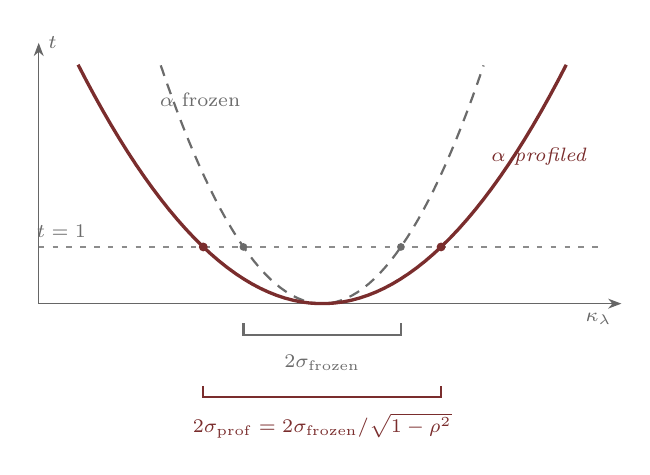
\begin{tikzpicture}[x=1.0cm, y=0.72cm]
  \draw[-{Stealth}, black!60] (-3.6,0) -- (3.8,0) node[below left, font=\scriptsize]{\kl};
  \draw[-{Stealth}, black!60] (-3.6,0) -- (-3.6,4.6) node[right, font=\scriptsize]{$t$};
  \draw[black!45, dash pattern=on 2pt off 3pt] (-3.6,1) -- (3.6,1) node[pos=0.04, above, font=\scriptsize, text=mut]{$t=1$};
  % frozen: t = x^2  (sigma=1)
  \draw[mut, thick, dash pattern=on 4pt off 3pt, domain=-2.05:2.05, samples=60] plot (\x, {\x*\x});
  \node[font=\scriptsize, text=mut] at (-1.55,3.6) {$\alpha$ frozen};
  % profiled: t = (x/1.51)^2
  \draw[accent, very thick, domain=-3.1:3.1, samples=60] plot (\x, {(\x/1.51)*(\x/1.51)});
  \node[font=\scriptsize\itshape, text=accent] at (2.75,2.6) {$\alpha$ profiled};
  % width markers at t=1
  \fill[mut] (-1,1) circle (1.4pt); \fill[mut] (1,1) circle (1.4pt);
  \fill[accent] (-1.51,1) circle (1.6pt); \fill[accent] (1.51,1) circle (1.6pt);
  \draw[mut, thick] (-1,-0.35) -- ++(0,-0.2) -- ++(2,0) -- ++(0,0.2);
  \node[font=\scriptsize, text=mut] at (0,-1.05) {$2\sigma_{\rm frozen}$};
  \draw[accent, thick] (-1.51,-1.45) -- ++(0,-0.2) -- ++(3.02,0) -- ++(0,0.2);
  \node[font=\scriptsize, text=accent] at (0,-2.15) {$2\sigma_{\rm prof}=2\sigma_{\rm frozen}/\sqrt{1-\rho^2}$};
\end{tikzpicture}
\caption{The profiled parabola is the frozen one flattened by exactly $(1-\rho^2)$; the $t\le1$ crossing moves
out by $1/\sqrt{1-\rho^2}$ (drawn for $\rho=0.75$, a factor 1.51).}
\label{fig:parab}
\end{figure}

\begin{takeaway}[The degeneracy-toy numbers \emph{are} this formula]
Exact for Gaussian likelihoods --- and the project's degeneracy-toy results are this formula evaluated: with the
10-feature set $\rho=0.65$, so $1/\sqrt{1-0.42}=1.31\times$ wider; with \mhh\ alone $\rho\approx0.997$ and the
same expression gives $12.8\times$. When we said ``dimensionality breaks the degeneracy,'' the mechanism was
literally: extra features give \kl\ an effect component that JES \emph{cannot} imitate, shrinking $\rho$,
un-tilting the ellipse, and closing the gap between slice and shadow.
\end{takeaway}

%---------------------------------------------------------------------
\subsection[The meaning of the profile likelihood ratio $\lambda(\kl)$]{The meaning of $\lambda(\kl)=L(\kl,\ahh(\kl))\,/\,L(\hat\kl,\hat\alpha)$}\label{sec:lambda}

\begin{qbox}[Question]
Is there an intuition for the definition of $\lambda(\kl)$?
\end{qbox}

Read it as a \textbf{courtroom with the best possible defense}:
\begin{itemize}
\item \textbf{Numerator} --- the hypothesis ``the coupling is \emph{this} \kl'' gets a defense attorney who may
  tune every systematic in its favor (within the Gaussian-constraint penalties): \emph{``the data look off
  because JES is $0.6\sigma$ high, $\tau$ES $0.3\sigma$ low\dots''}. $L(\kl,\ahh(\kl))$ is the \textbf{best
  case that can possibly be made} for this \kl.
\item \textbf{Denominator} --- the best case for the \textbf{champion}: the globally best $(\hat\kl,\hat\alpha)$,
  the hypothesis that explains the data best of all.
\item $\lambda$ is then a number in $[0,1]$: \emph{how close does this \kl's best defense come to the
  champion's?} Near 1 $\to$ it explains the data essentially as well; there are no grounds to exclude it; it is
  in the interval. Small $\to$ even with every systematic maximally in its favor, it still fails; excluded. And
  $t=-2\ln\lambda$ converts ``how much worse'' onto the $\chi^2$ scale (Wilks), which is what makes
  $t\le1\leftrightarrow68\%$ a universal calibration.
\end{itemize}

Why each ingredient is there:
\begin{itemize}
\item \textbf{Why a ratio at all?} An absolute likelihood value is meaningless --- it depends on
  normalizations, units, and modeling constants that have nothing to do with \kl. Dividing by the global
  maximum cancels all of that and leaves a pure \emph{relative} plausibility. It is also not arbitrary: for
  simple hypotheses the likelihood ratio is provably the most powerful test (Neyman--Pearson); $\lambda$ is its
  canonical generalization to hypotheses with unknown nuisances (the generalized likelihood-ratio test).
\item \textbf{Why maximize over $\alpha$ (double-hat) instead of freezing it?} Freezing $\alpha$ at the
  champion's $\hat\alpha$ rigs the trial --- the nuisance values were chosen to fit the \emph{champion}, so
  every other \kl\ gets judged with a defense tuned for someone else (that is the too-narrow slice interval of
  Fig.~\ref{fig:slice}, and it under-covers). Profiling gives \textbf{each hypothesis its own best defense},
  and that is precisely what buys the frequentist guarantee: the interval covers at the stated rate \emph{no
  matter what the true $\alpha$ is} (asymptotically), because no \kl\ was excluded that some legitimate
  $\alpha$ could have rescued.
\item \textbf{Geometric reading:} the numerator, as a function of \kl, is the likelihood \textbf{along the
  ridge} --- so $t(\kl)$ is simply \emph{the height of the tilted valley's floor above the global minimum}. The
  profiled parabola of Fig.~\ref{fig:parab} is nothing but the valley floor seen edge-on from the \kl\ axis.
\end{itemize}

\begin{keybox}[How the two questions join up]
The $\ahh$ in the numerator of $\lambda$ \emph{is} the ridge in Fig.~\ref{fig:slice}. Evaluating $\lambda$ at
some \kl\ \emph{is} the act of sliding down to the ridge --- the numerator does the rescuing, the denominator
sets the standard, and the tilt ($\rho$) decides how much rescuing is possible, which is exactly how much the
interval widens.
\end{keybox}

%=====================================================================
\section{The four off-shell (R2) assumptions, and how they break per channel}\label{sec:assumptions}

\begin{qbox}[Question]
Can you elaborate on the meanings of these assumptions in the off-shell measurement (a fixed order in
$\alpha$; ignores kinematics for $|\alpha|<1$; assumes factorization / no non-factorizable NPs; doesn't exploit
joint likelihood ratios) --- and how do they break for $\lambda$ in the HH analysis, separately for \bbtt,
\bbgg, \fourb?
\end{qbox}

\paragraph{Provenance.} As Lesson 1 flags, that list is \textbf{the R4 group's critique of R2} --- how the
refinable/GOLLUM papers characterize the ATLAS approach. ATLAS would fairly reply that for clean $4\ell$ these
approximations were validated as adequate. What each means mechanically (all four are visible in
Fig.~\ref{fig:pins}):

\begin{enumerate}
\item \textbf{``Two classifiers per NP'' $+$ ``fixed order in $\alpha$.''} R2 trains classifiers only at the
  $\pm1\sigma$ anchors: $w_+(x)$ and $w_-(x)$ per NP per process. The entire $\alpha$-dependence of each
  event's weight is then \textbf{pinned by just those two numbers}, threaded through the fixed poly-exp family
  (Sec.~\ref{sec:pins}). ``Fixed order'' $=$ the \emph{shape of the $\alpha$-curve} is chosen a priori, not
  learned. If the true per-event response is non-monotone in $\alpha$, or has genuine curvature the family
  cannot express, it is silently truncated --- with \textbf{zero assigned uncertainty} for being wrong.
\item \textbf{``Ignores kinematics for $|\alpha|<1$.''} The $x$-dependence enters \emph{only} through the two
  anchor weights. At $\alpha=0.4$, event $e$'s weight is a fixed interpolation of $w_+(x_e)$ and $w_-(x_e)$ ---
  \textbf{no simulation at intermediate $\alpha$ ever informs it}. The hidden assumption: the \emph{pattern} of
  the deformation across phase space at fractional $\alpha$ is the same as at $\pm1\sigma$, just scaled. When
  the response chain is nonlinear (reconstruction thresholds, migrations), different regions of phase space
  ``turn on'' at different $\alpha$ --- and the interpolation cannot know.
\item \textbf{``Assumes factorization.''} $w(x,\alpha)=\prod_m w_m(x,\alpha_m)$ --- each NP acts independently
  on the density; no cross-terms. True when NPs touch different objects (lepton ES $\times$ lumi). False when
  two NPs feed the \emph{same reconstructed quantity}.
\item \textbf{``Doesn't exploit joint likelihood ratios.''} Every anchor classifier is trained \textbf{in
  isolation} --- one (NP, direction, process) at a time. Nothing enforces consistency across them, there is no
  statistical pooling across variations, and each carries its \emph{own} independent MC-stat noise (this is
  C6's multiplier). R4 instead fits \textbf{one} parametric surface
  $\log w(x,\alpha)=\sum_A\alpha_A\,\hat\Delta_A(x)$ to \emph{all} variation samples jointly --- shared
  statistics, consistent correlations, cross-terms included at chosen order.
\end{enumerate}

\paragraph{Channel-by-channel breakage.} (\bbtt\ claims are grounded in this project's doc/CMS note;
\textbf{\bbgg\ and \fourb\ are from the standard structure of those analyses --- verify against the specific
ATLAS/CMS analyses before quoting.})

\begin{table}[htbp]\centering\footnotesize
\begin{tabular}{@{}p{0.14\textwidth}p{0.27\textwidth}p{0.25\textwidth}p{0.26\textwidth}@{}}
\toprule
\textbf{Assumption} & \textbf{\bbtt} & \textbf{\bbgg} & \textbf{\fourb}\\
\midrule
fixed order in $\alpha$ &
\textbf{stressed} --- $\tau$ES propagates through MET$\to$SVfit$\to m_{\tau\tau}$, a nonlinear likelihood-based
estimator; JES drives category/selection migrations &
mild --- photon ES is sub-percent (linear regime); only the $b$-side JES has room to misbehave &
\textbf{worst} --- JES/JER can \emph{flip the jet pairing} (which jets form $h_1,h_2$): per-event response is
discontinuous in $\alpha$, outside any smooth family\\
\addlinespace[3pt]
kinematics at $|\alpha|<1$ &
\textbf{stressed} --- $\tau$ES is $p_{\rm T}$- and decay-mode-dependent; the deformation \emph{pattern} at
fractional $\alpha$ $\ne$ scaled anchor pattern &
mild --- small, nearly linear responses; anchors suffice &
\textbf{stressed} --- $b$-jet trigger turn-ons and pairing migrations cross thresholds at \emph{different}
$\alpha$ for different event subsets\\
\addlinespace[3pt]
factorization &
\textbf{broken by construction} --- JES$\times\tau$ES both feed $\mhh=m(b\bar b+\tau\tau)$ (C5); plus $b$-tag
SFs are $p_{\rm T}$-binned, so JES moves events across SF bins (JES$\times b$-tag) &
largely OK --- PES$\times$JES negligible (PES tiny); residual JES$\times b$-tag mild &
\textbf{worst} --- 11 JES sources $\times$ JER $\times$ 4 $b$-tags all act on the \emph{same four jets} and the
same $m_{4b}/m_{h_1}/m_{h_2}$; pairing couples them jointly\\
\addlinespace[3pt]
joint LRs &
\textbf{expensive to forgo} --- $\sim$40 NPs $\times\sim$7 processes $\times$ 2 anchors $\times$ ensemble
$\approx$ thousands of independent nets, each noisy on the smallest $\pm1\sigma$ samples (C6, C2) &
fewer NPs; $\pm1\sigma$ samples still finite --- pooling helps, stakes lower &
\textbf{expensive} --- many NPs \emph{plus} the background itself is a learned reweighting ($2b{\to}4b$ /
FvT-style NN with bootstrap ensembles); nobody has jointly treated a learned background $+$ learned systematics\\
\addlinespace[3pt]
(channel wildcard) &
data-driven QCD/fakes with no density (C3); \texttt{THU\_HH} POI-coupling (C4) &
continuum $\gamma\gamma$ fit in $m_{\gamma\gamma}$ sidebands $\to$ the ``spurious-signal'' NP is a
\textbf{discrete model choice}, not a continuous $\alpha$ --- does not map to morphing at all &
dominant QCD estimate is itself a NN reweighting $\to$ its systematic is a nuisance \emph{on a learned object};
C3 in its hardest form\\
\bottomrule
\end{tabular}
\caption{The four R2 assumptions across the three main HH channels.}
\label{tab:channels}
\end{table}

\begin{takeaway}[The pattern worth internalizing]
\textbf{\bbgg\ mostly inherits R2's assumptions safely} (its hard problem is tiny yields, not morphing);
\textbf{\bbtt\ breaks factorization and stresses the fixed-form interpolation} (via the SVfit chain);
\textbf{\fourb\ breaks everything at once} (combinatorics make the response non-smooth, correlated, and the
background is itself learned). That ordering --- $\gamma\gamma$ easiest, $\tau\tau$ middle, $4b$ hardest --- is
also the order in which the R2 recipe ports without modification.
\end{takeaway}

%=====================================================================
\section{The upgrades: R3 (GP morphing) and R4 (refinable surrogate)}\label{sec:upgrades}

\subsection{R3: Gaussian-Process morphing --- mechanics, comparison, deployment for \kl}\label{sec:gp}

\begin{qbox}[Question]
Can you help me understand how R3 Gaussian-Process morphing works, and how it compares with what was done in
off-shell, with our application to $\lambda$ in mind? \emph{(Context: R3 is led by the developer of the NSBI
repo we've been working with.)}
\end{qbox}

\paragraph{Mechanics, single NP first.} There are simulations at a few anchor settings of $\alpha$ --- say
$-2\sigma,-1\sigma,0,+1\sigma,+2\sigma$. The quantity to morph (a bin's content ratio, or in the unbinned case
a per-event weight / the coefficient functions of the weight) is an unknown function $\Delta(\alpha)$. Instead
of \emph{assuming} poly-exp, place a \textbf{Gaussian-Process prior} on it --- ``$\Delta$ is some smooth
function, with correlations over $\alpha$ set by a kernel $k(\alpha,\alpha')$'' --- and \textbf{condition on
the anchors}. The posterior gives two things at every $\alpha$:
\begin{itemize}
\item a \textbf{mean} --- the interpolated morphing the fit uses (playing exactly the role poly-exp played), and
\item a \textbf{covariance} --- \emph{how uncertain the interpolation itself is}: small at anchors, growing
  between and especially \textbf{beyond} them.
\end{itemize}
That covariance is the unique feature: it enters the fit as extra constrained parameters ($\gamma$) --- so if
the fit pulls a nuisance into a region where the morphing is poorly determined, the likelihood
\textbf{automatically pays a penalty} instead of trusting an assumption. This is ``honest morphing'' --- study
\#9 of the challenges note, and the direct mitigation of the \emph{tighter-but-mis-covering} failure mode.

\paragraph{Multi-NP: two R2 assumptions die at once.} The GP's input can be the \emph{vector} $\alpha$, and the
anchors \textbf{need not sit on the axes} --- a simulated sample with JES and $\tau$ES shifted \emph{together}
is just another anchor point. The kernel then learns the joint response surface directly: \textbf{no
factorization assumed} (C5 handled by data, not by ansatz) and \textbf{no fixed order} (non-parametric). A
subtle bonus relevant to C6: anchor points are themselves noisy (finite $\pm1\sigma$ MC), and GP regression
naturally takes per-anchor noise --- so the MC-stat of the \emph{variation samples} feeds coherently into the
interpolation band rather than being handled by a separate bolted-on estimator.

\begin{table}[htbp]\centering\small
\begin{tabular}{@{}p{0.30\textwidth}p{0.30\textwidth}p{0.32\textwidth}@{}}
\toprule
 & \textbf{R2 off-shell (poly-exp)} & \textbf{R3 (GP)}\\
\midrule
functional form in $\alpha$ & fixed family, pinned by $\pm1\sigma$ & learned from anchors, non-parametric\\
cross-terms (JES$\times\tau$ES) & excluded (factorized product) & included via off-axis anchors $+$ joint kernel\\
interpolation error & \textbf{assumed zero} & \textbf{quantified} (posterior cov $\to$ constrained $\gamma$)\\
anchor MC-stat & separate estimator (the contested C6) & enters as GP observation noise\\
cost / risk & cheap, rigid & kernel choice $=$ injected bias; needs more anchor samples (esp.\ off-axis);
  pre-publication\\
\bottomrule
\end{tabular}
\caption{Off-shell interpolation vs GP morphing, term by term.}
\label{tab:gp}
\end{table}

\paragraph{For \kl\ specifically.} Challenge C1 says morphing accuracy \emph{directly sets} the \kl\
uncertainty, because the systematics deform the observable that carries the signal. That is precisely the
regime where an \emph{assumed-perfect} interpolation is dangerous and an honest band is worth its width. The
pragmatic deployment is not ``GP everything'' --- it is: keep the R2 skeleton, and \textbf{swap poly-exp $\to$
GP for the top-impact, cross-term-prone NPs} (the JES sources and $\tau$ES components feeding \mhh), requesting
a handful of off-axis anchor samples for exactly those pairs. Note the GP does \emph{not} by itself solve C4
--- the POI-coupling of \texttt{THU\_HH} needs the per-component decomposition first; GP can then morph each
component honestly.

\paragraph{The sociology is a real planning input.} R3's Sandesara is both the off-shell lead author and the
developer of the upstream toolkit this project builds on, with \texttt{pyhf-gpsys} headed for the standard
stacks. So \textbf{R3 is the low-friction, in-ecosystem upgrade path} (likely with direct support in the very
framework in use), while R4 is an external stack --- which sets up the next question.

%---------------------------------------------------------------------
\subsection{R4 is \emph{not} generative (not normalizing flows) --- and why that is good news}\label{sec:r4}

\begin{qbox}[Question]
R4 is a generative-based approach (normalizing flows) --- does that apply to ours (training a classifier to
learn the density ratio) at all? \emph{(Context: R4 is by another group, despite seeming to have many
advantages.)}
\end{qbox}

This premise deserves a careful correction, because it changes the applicability answer completely. Checked
against the lessons \emph{and} the sources: R4 ---
\href{https://arxiv.org/abs/2406.19076}{``Refinable modeling for unbinned SMEFT analyses''} (MLST 6 015007) and
its application paper
\href{https://arxiv.org/abs/2505.05544}{``Unbinned inclusive cross-section measurements with machine-learned
systematic uncertainties''} (PRD 112 052006) --- is \textbf{not} flow-based or generative. It learns
\textbf{machine-learned surrogates of the likelihood \emph{ratio}}, with the coefficient functions of the
ansatz
\begin{equation}
\log\frac{\sigma(\alpha)}{\sigma(0)}\Big|_x\;=\;\sum_A \alpha_A\,\hat\Delta_A(x)
\qquad\text{($A$ ranging over linear, quadratic, and cross-terms)}
\end{equation}
fit by a \textbf{tree-boosting algorithm} (and NN variants) trained with cross-entropy-style losses on the
variation samples. That is \emph{discriminative ratio estimation} --- the same statistical trick as the CARL
classifiers used throughout this project --- just organized as one \textbf{joint, $\alpha$-parametric} fit
instead of independent anchor pairs.

So the answer to ``does it apply to ours at all?'' is: \textbf{it applies maximally --- it \emph{is} our
approach, upgraded.} Porting R4's idea into the pipeline means replacing
\begin{center}
\{2 independent classifiers per NP\} $+$ \{fixed poly-exp bridge\}
\end{center}
with
\begin{center}
\{one set of coefficient networks $\hat\Delta_A(x)$ per process, fit jointly to \emph{all} variation samples,\\
with cross-terms ($A=$ pairs) included at whatever order is affordable --- ``refinable''\}.
\end{center}
No generative modeling, no flows, no change to the reference-hypothesis trick or the fit --- just a
better-parameterized ratio head trained with machinery already in place.

\paragraph{Where the flows association likely came from} (worth untangling, since both live in this program):
\textbf{flows appear in the \emph{background-density} thread, not the systematics thread} --- ABCDnn (the
neural autoregressive flow learning a data-driven QCD/fakes density, challenge C3) and the FlowNF-style toy
cited once alongside GOLLUM in the C4 verdict box of the challenges note. Those are generative because their
job is to \emph{manufacture a density that does not exist}. R4's job is to \emph{deform a density you already
have} --- a ratio problem, solved discriminatively.

\begin{takeaway}[Resolving R3-vs-R4 without choosing]
\textbf{R4 is an idea implementable inside our own stack} (a joint parametric ratio head --- no dependency on
GOLLUM), while \textbf{R3 is an ecosystem component} likely to arrive with native support in the framework in
use. The hybrid already on record --- R2 skeleton $+$ R4-style joint/cross-term ansatz where factorization
breaks $+$ R3-style GP band where interpolation honesty matters most --- uses each group's contribution where
it is strongest, without adopting either wholesale.
\end{takeaway}

%=====================================================================
\section{Synthesis: mapping this Q\&A onto the challenge list}

\begin{keybox}[One box to remember]
\begin{itemize}[leftmargin=1.2em]
\item \textbf{C1 (\kl--systematic degeneracy)} $=$ the \emph{tilt} $\rho$ of Sec.~\ref{sec:slice}; the widening
  is exactly $1/\sqrt{1-\rho^2}$; dimensionality shrinks $\rho$.
\item \textbf{C2 (NP scaling)} $=$ the count of Family-2 objects (Table~\ref{tab:families}):
  $2\times N_{\rm NP}\times N_{\rm comp}\times$ ensemble.
\item \textbf{C4 (POI-coupled theory)} $=$ the green/red boundary of Sec.~\ref{sec:green} leaking; in the
  pin picture, the pins themselves would have to move with \kl.
\item \textbf{C5 (cross-terms)} $=$ multiplying per-NP pin-curves (Fig.~\ref{fig:pins}); relaxed by R4's joint
  ansatz or R3's off-axis anchors.
\item \textbf{C6 (MC-stat of learned ratios)} $=$ each pin-pair trained in isolation carrying its own noise;
  relaxed by joint training (R4), GP anchor-noise (R3), or an analytic estimator (wifi).
\end{itemize}
\end{keybox}

\begin{thebibliography}{9}\small
\bibitem{atlas} ATLAS Collaboration (J.~Sandesara \emph{et al.}), \emph{An implementation of neural
  simulation-based inference for parameter estimation in ATLAS}, arXiv:2412.01600, Rep.\ Prog.\ Phys.\ 88
  (2025). The R2 recipe: per-event factorized weights, $\pm1\sigma$ anchor classifiers, poly-exp interpolation.
\bibitem{gollumM} R.~Schöfbeck \emph{et al.}, \emph{Refinable modeling for unbinned SMEFT analyses},
  arXiv:2406.19076, MLST 6 015007 (2025). The R4 method: tree-boosted, $\alpha$-parametric likelihood-ratio
  surrogates (discriminative, \emph{not} flows).
\bibitem{gollumA} R.~Schöfbeck \emph{et al.}, \emph{Unbinned inclusive cross-section measurements with
  machine-learned systematic uncertainties}, arXiv:2505.05544, PRD 112 052006 (2025). R4 tested (GOLLUM), incl.\
  on the FAIR Universe benchmark.
\bibitem{gpsys} K.~Cranmer, M.~Feickert, L.~Heinrich, A.~Held, J.~Sandesara, \emph{HistFactory v2 /
  Gaussian-Process systematic morphing}, SBI Blueprint (Feb 2026); \url{https://github.com/pyhf/pyhf-gpsys}.
  The R3 mechanism: GP over anchors, posterior covariance as interpolation uncertainty.
\bibitem{chal} \emph{New challenges for an NSBI measurement of \kl\ in HH$\to$\bbtt}, this workspace,
  \texttt{2026-06-20-klambda-nsbi-vs-offshell-challenges.pdf} --- challenge labels C1--C6, the maturity/risk
  matrix, and the width and compute analyses referenced here.
\end{thebibliography}

\end{document}
